\subsubsection{LP distributions}

This section contains the MVA output plots for the LP dataset for $m_H$=115, 120, 130, 140, 150, 160, 200 GeV analyses split in opposte and same flavor, 
0-jet and 1-jet bin (Figures~\ref{fig:lp_mva_115}-\ref{fig:lp_mva_200}).

\begin{figure}[!hbtp]
\centering
\subfigure[]{
\centering
\label{subfig:lp_mva_115_0j_of}
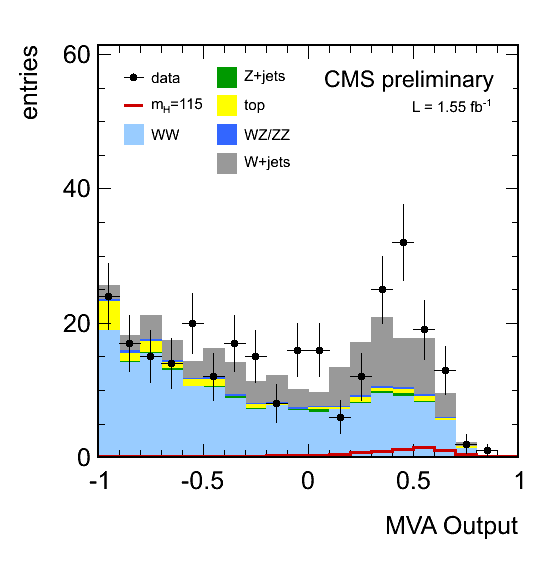
\includegraphics[width=.40\textwidth]{lp_figures/histo_mva_115_0j_of.png}}
\subfigure[]{
\centering
\label{subfig:lp_mva_115_0j_sf}
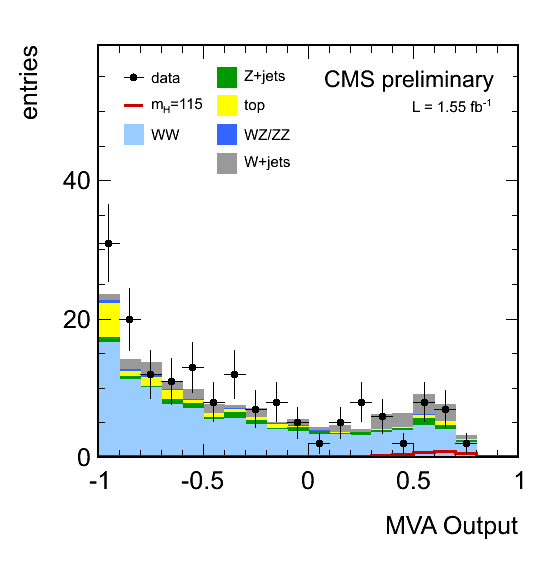
\includegraphics[width=.40\textwidth]{lp_figures/histo_mva_115_0j_sf.png}}\\
\subfigure[]{
\centering
\label{subfig:lp_mva_115_1j_of}
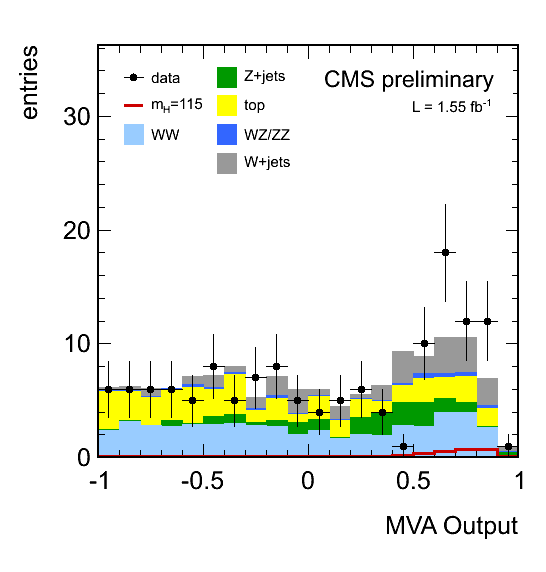
\includegraphics[width=.40\textwidth]{lp_figures/histo_mva_115_1j_of.png}}
\subfigure[]{
\centering
\label{subfig:lp_mva_115_1j_sf}
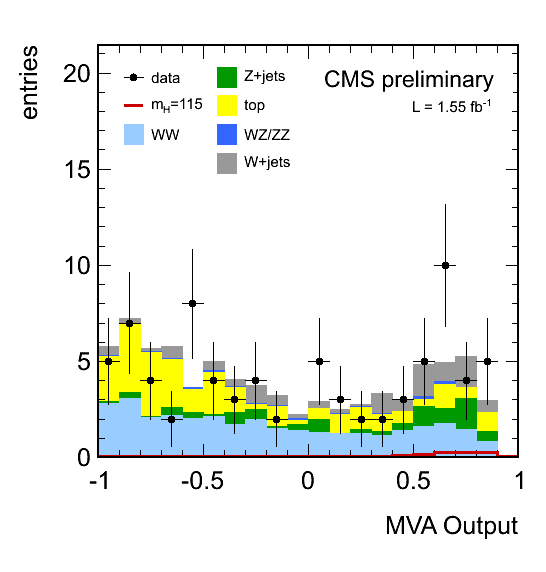
\includegraphics[width=.40\textwidth]{lp_figures/histo_mva_115_1j_sf.png}}
\caption{
MVA output for $m_H$=115 GeV LP analysis: 
0-jet OF \subref{subfig:lp_mva_115_0j_of},
0-jet SF \subref{subfig:lp_mva_115_0j_sf},
1-jet OF \subref{subfig:lp_mva_115_1j_of},
1-jet SF \subref{subfig:lp_mva_115_1j_sf}
.}
\label{fig:lp_mva_115}
\end{figure}

\begin{figure}[!hbtp]
\centering
\subfigure[]{
\centering
\label{subfig:lp_mva_120_0j_of}
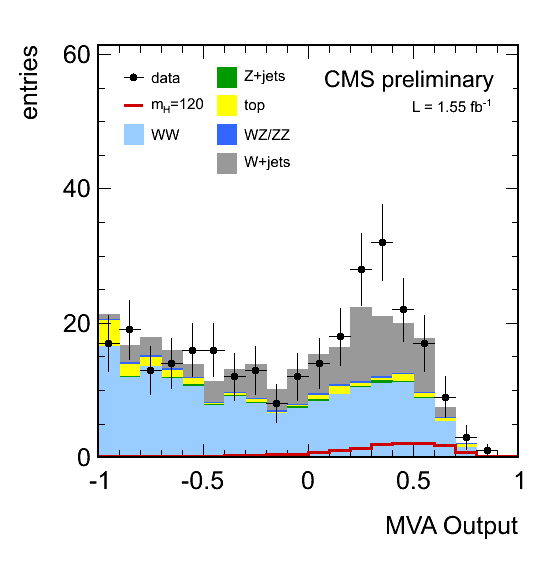
\includegraphics[width=.40\textwidth]{lp_figures/histo_mva_120_0j_of.png}}
\subfigure[]{
\centering
\label{subfig:lp_mva_120_0j_sf}
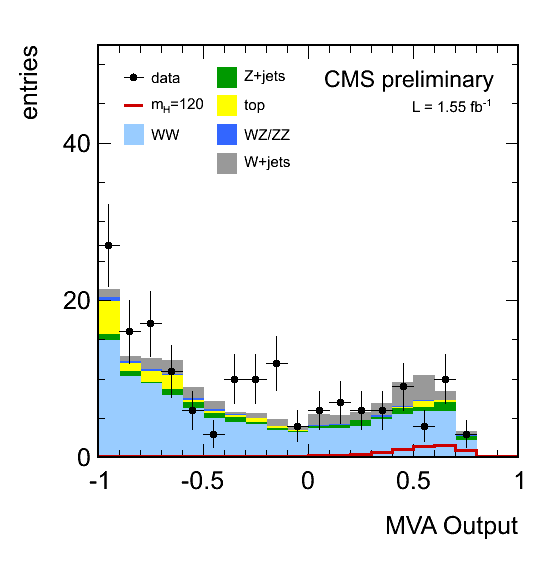
\includegraphics[width=.40\textwidth]{lp_figures/histo_mva_120_0j_sf.png}}\\
\subfigure[]{
\centering
\label{subfig:lp_mva_120_1j_of}
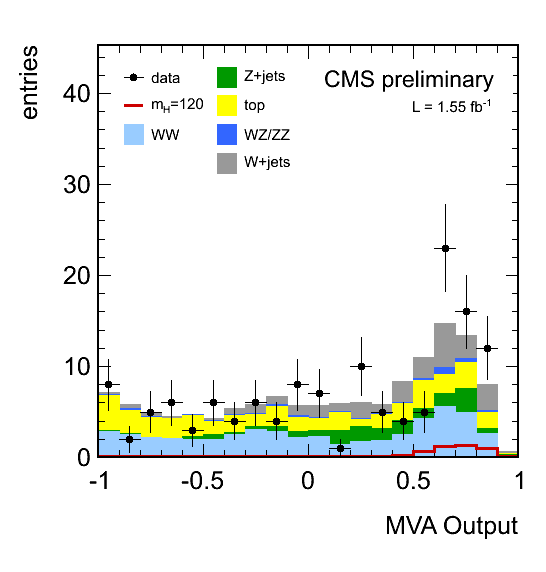
\includegraphics[width=.40\textwidth]{lp_figures/histo_mva_120_1j_of.png}}
\subfigure[]{
\centering
\label{subfig:lp_mva_120_1j_sf}
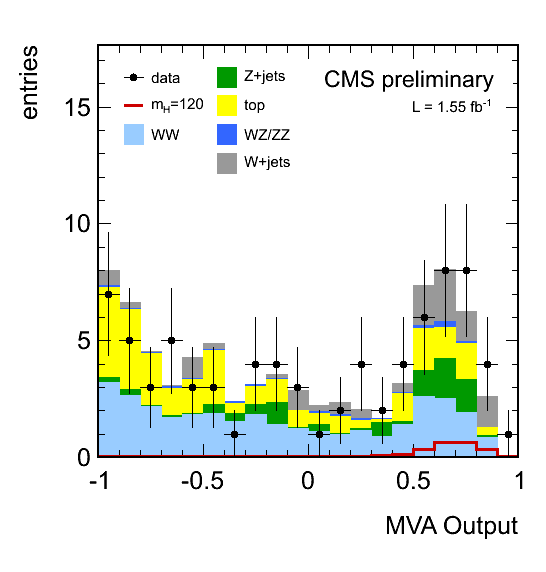
\includegraphics[width=.40\textwidth]{lp_figures/histo_mva_120_1j_sf.png}}
\caption{
MVA output for $m_H$=120 GeV LP analysis: 
0-jet OF \subref{subfig:lp_mva_120_0j_of},
0-jet SF \subref{subfig:lp_mva_120_0j_sf},
1-jet OF \subref{subfig:lp_mva_120_1j_of},
1-jet SF \subref{subfig:lp_mva_120_1j_sf}
.}
\label{fig:lp_mva_120}
\end{figure}

\begin{figure}[!hbtp]
\centering
\subfigure[]{
\centering
\label{subfig:lp_mva_130_0j_of}
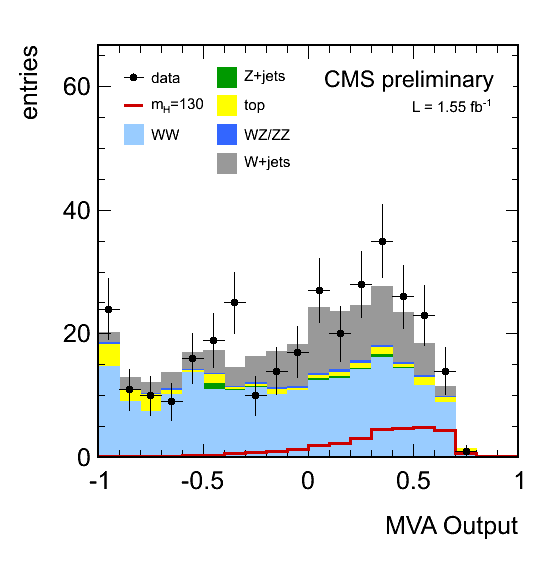
\includegraphics[width=.40\textwidth]{lp_figures/histo_mva_130_0j_of.png}}
\subfigure[]{
\centering
\label{subfig:lp_mva_130_0j_sf}
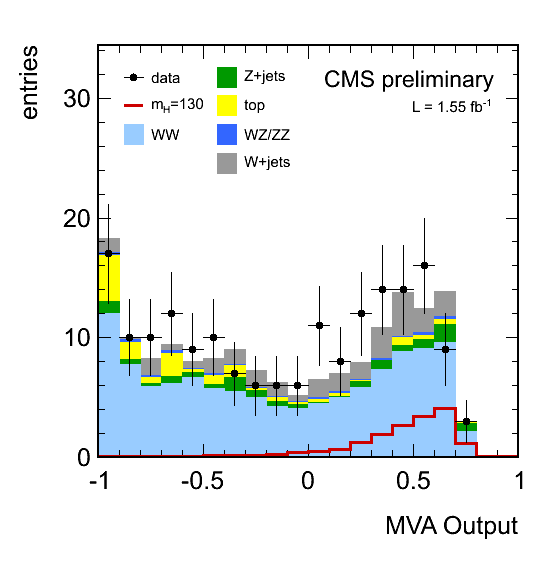
\includegraphics[width=.40\textwidth]{lp_figures/histo_mva_130_0j_sf.png}}\\
\subfigure[]{
\centering
\label{subfig:lp_mva_130_1j_of}
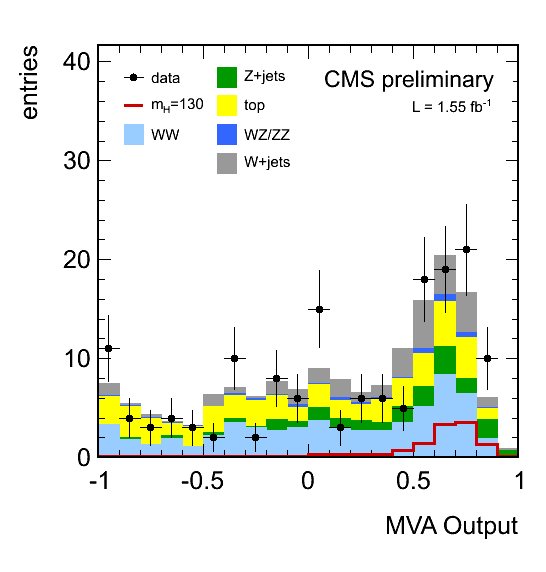
\includegraphics[width=.40\textwidth]{lp_figures/histo_mva_130_1j_of.png}}
\subfigure[]{
\centering
\label{subfig:lp_mva_130_1j_sf}
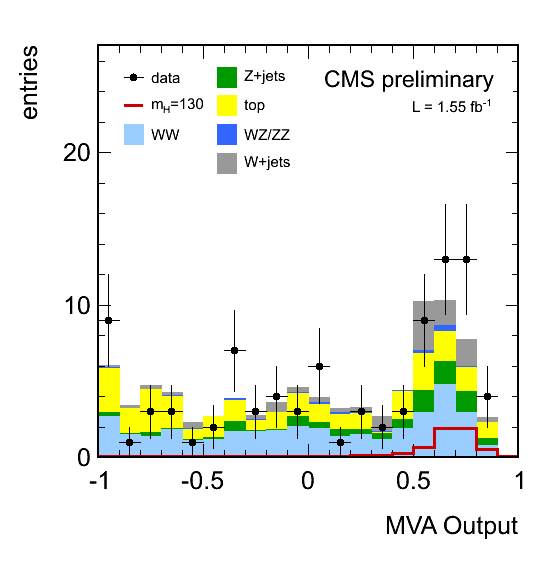
\includegraphics[width=.40\textwidth]{lp_figures/histo_mva_130_1j_sf.png}}
\caption{
MVA output for $m_H$=130 GeV LP analysis: 
0-jet OF \subref{subfig:lp_mva_130_0j_of},
0-jet SF \subref{subfig:lp_mva_130_0j_sf},
1-jet OF \subref{subfig:lp_mva_130_1j_of},
1-jet SF \subref{subfig:lp_mva_130_1j_sf}
.}
\label{fig:lp_mva_130}
\end{figure}

\begin{figure}[!hbtp]
\centering
\subfigure[]{
\centering
\label{subfig:lp_mva_140_0j_of}
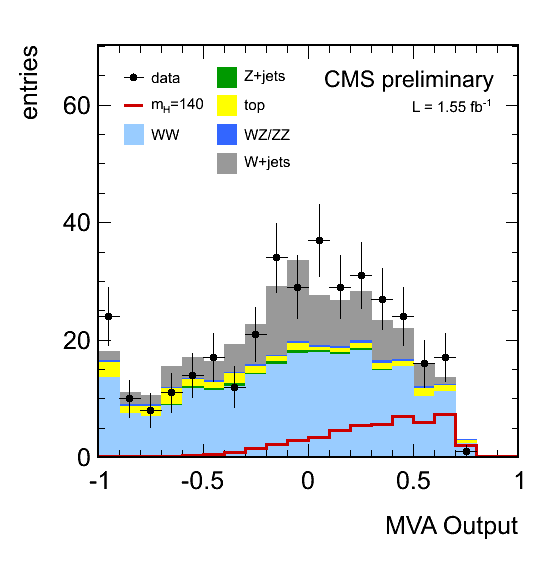
\includegraphics[width=.40\textwidth]{lp_figures/histo_mva_140_0j_of.png}}
\subfigure[]{
\centering
\label{subfig:lp_mva_140_0j_sf}
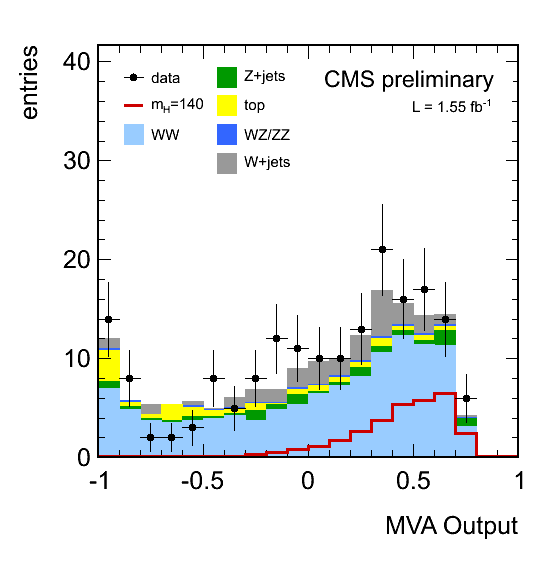
\includegraphics[width=.40\textwidth]{lp_figures/histo_mva_140_0j_sf.png}}\\
\subfigure[]{
\centering
\label{subfig:lp_mva_140_1j_of}
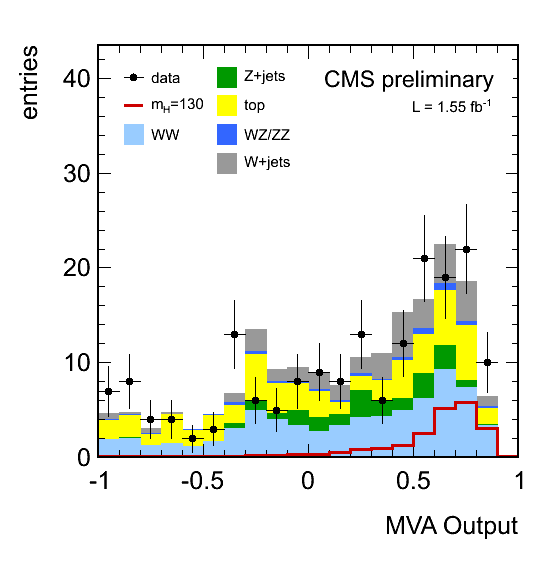
\includegraphics[width=.40\textwidth]{lp_figures/histo_mva_140_1j_of.png}}
\subfigure[]{
\centering
\label{subfig:lp_mva_140_1j_sf}
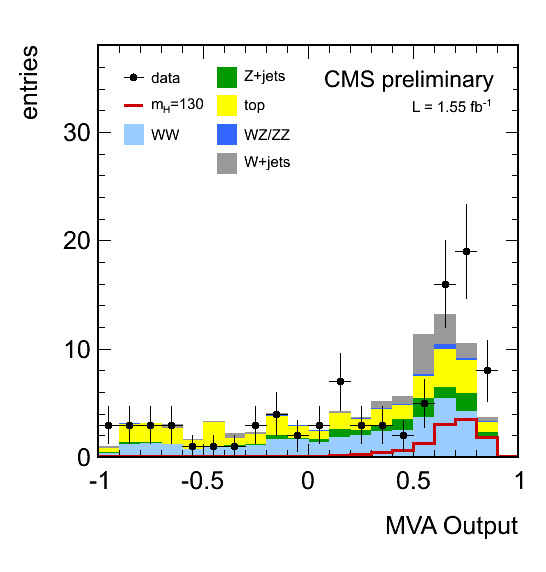
\includegraphics[width=.40\textwidth]{lp_figures/histo_mva_140_1j_sf.png}}
\caption{
MVA output for $m_H$=140 GeV LP analysis: 
0-jet OF \subref{subfig:lp_mva_140_0j_of},
0-jet SF \subref{subfig:lp_mva_140_0j_sf},
1-jet OF \subref{subfig:lp_mva_140_1j_of},
1-jet SF \subref{subfig:lp_mva_140_1j_sf}
.}
\label{fig:lp_mva_140}
\end{figure}

\begin{figure}[!hbtp]
\centering
\subfigure[]{
\centering
\label{subfig:lp_mva_150_0j_of}
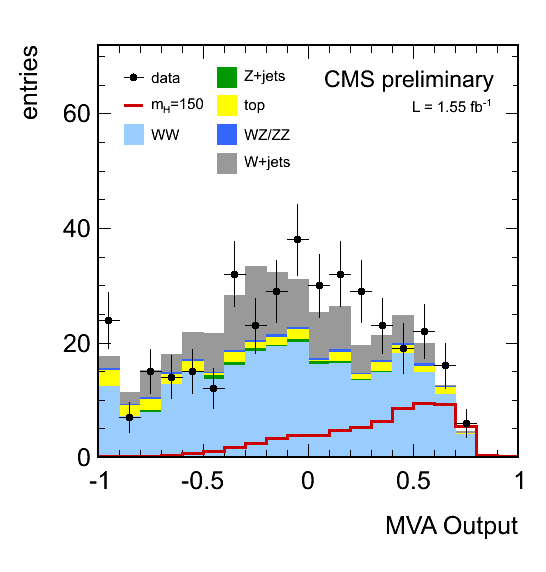
\includegraphics[width=.40\textwidth]{lp_figures/histo_mva_150_0j_of.png}}
\subfigure[]{
\centering
\label{subfig:lp_mva_150_0j_sf}
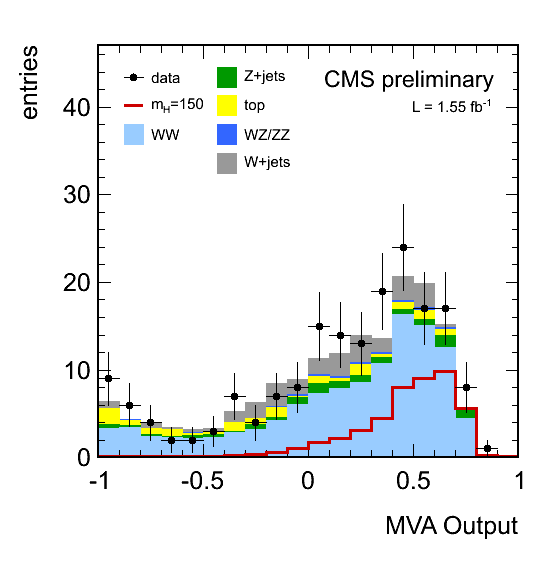
\includegraphics[width=.40\textwidth]{lp_figures/histo_mva_150_0j_sf.png}}\\
\subfigure[]{
\centering
\label{subfig:lp_mva_150_1j_of}
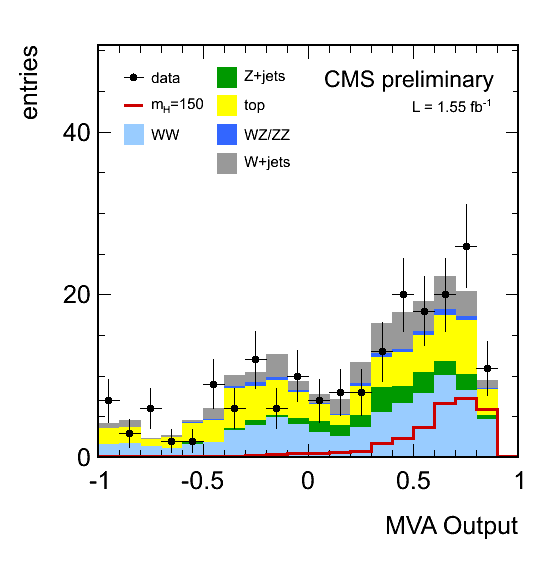
\includegraphics[width=.40\textwidth]{lp_figures/histo_mva_150_1j_of.png}}
\subfigure[]{
\centering
\label{subfig:lp_mva_150_1j_sf}
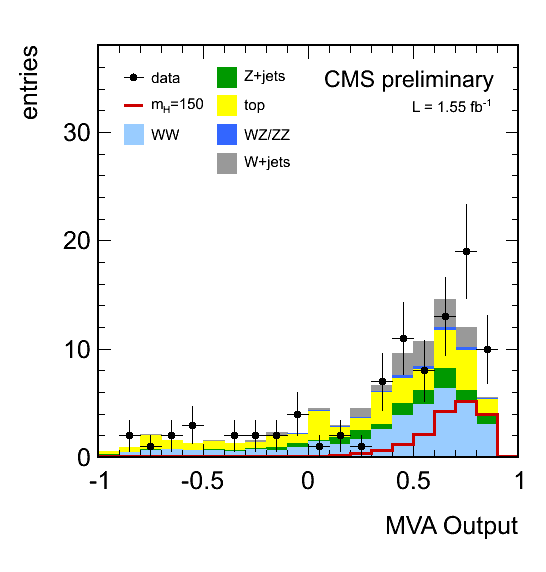
\includegraphics[width=.40\textwidth]{lp_figures/histo_mva_150_1j_sf.png}}
\caption{
MVA output for $m_H$=150 GeV LP analysis: 
0-jet OF \subref{subfig:lp_mva_150_0j_of},
0-jet SF \subref{subfig:lp_mva_150_0j_sf},
1-jet OF \subref{subfig:lp_mva_150_1j_of},
1-jet SF \subref{subfig:lp_mva_150_1j_sf}
.}
\label{fig:lp_mva_150}
\end{figure}

\begin{figure}[!hbtp]
\centering
\subfigure[]{
\centering
\label{subfig:lp_mva_160_0j_of}
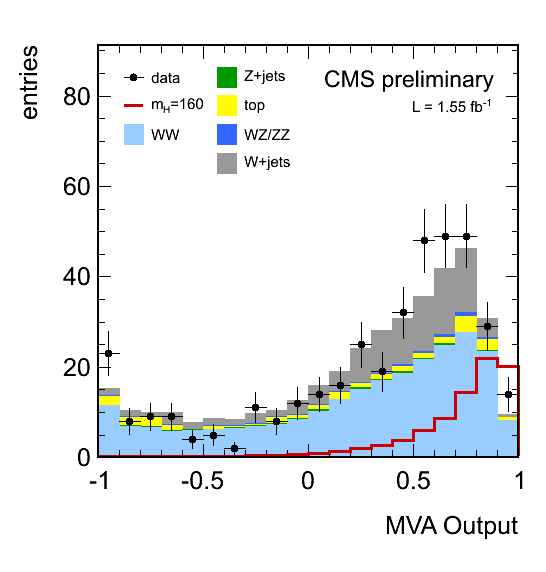
\includegraphics[width=.40\textwidth]{lp_figures/histo_mva_160_0j_of.png}}
\subfigure[]{
\centering
\label{subfig:lp_mva_160_0j_sf}
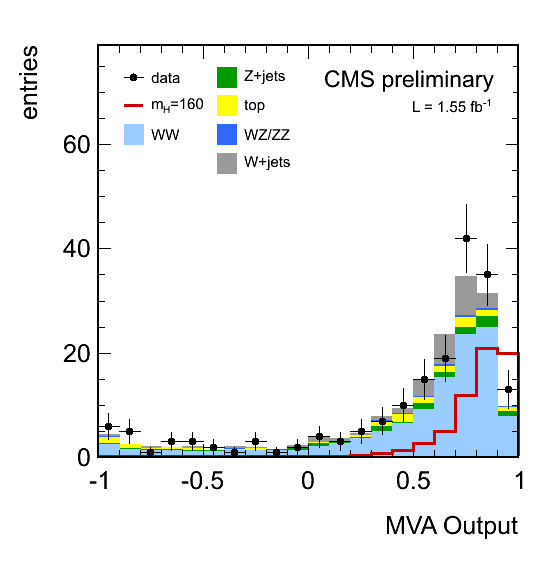
\includegraphics[width=.40\textwidth]{lp_figures/histo_mva_160_0j_sf.png}}\\
\subfigure[]{
\centering
\label{subfig:lp_mva_160_1j_of}
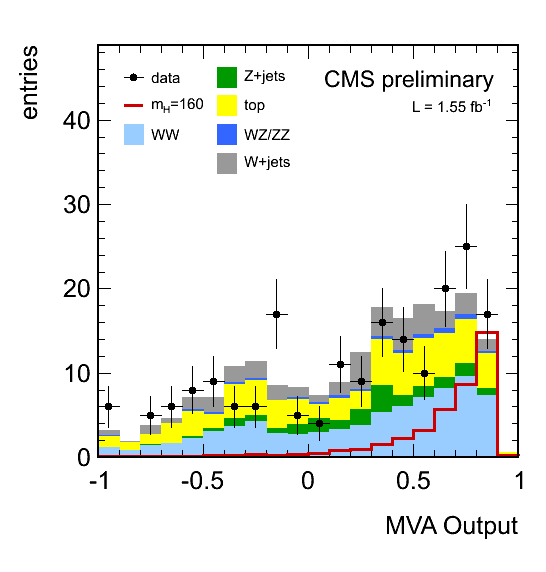
\includegraphics[width=.40\textwidth]{lp_figures/histo_mva_160_1j_of.png}}
\subfigure[]{
\centering
\label{subfig:lp_mva_160_1j_sf}
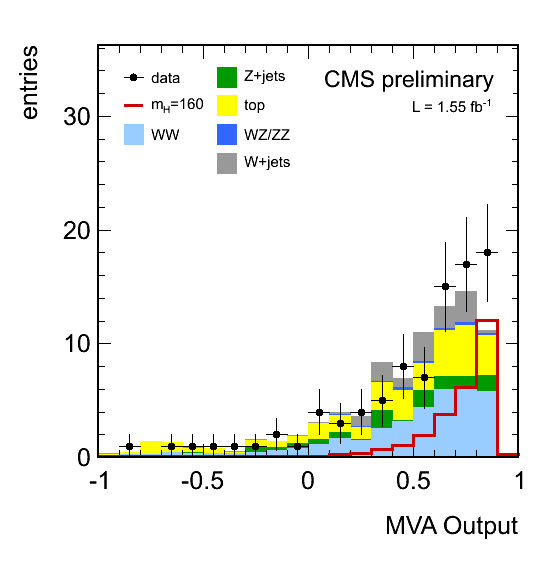
\includegraphics[width=.40\textwidth]{lp_figures/histo_mva_160_1j_sf.png}}
\caption{
MVA output for $m_H$=160 GeV LP analysis: 
0-jet OF \subref{subfig:lp_mva_160_0j_of},
0-jet SF \subref{subfig:lp_mva_160_0j_sf},
1-jet OF \subref{subfig:lp_mva_160_1j_of},
1-jet SF \subref{subfig:lp_mva_160_1j_sf}
.}
\label{fig:lp_mva_160}
\end{figure}

\begin{figure}[!hbtp]
\centering
\subfigure[]{
\centering
\label{subfig:lp_mva_200_0j_of}
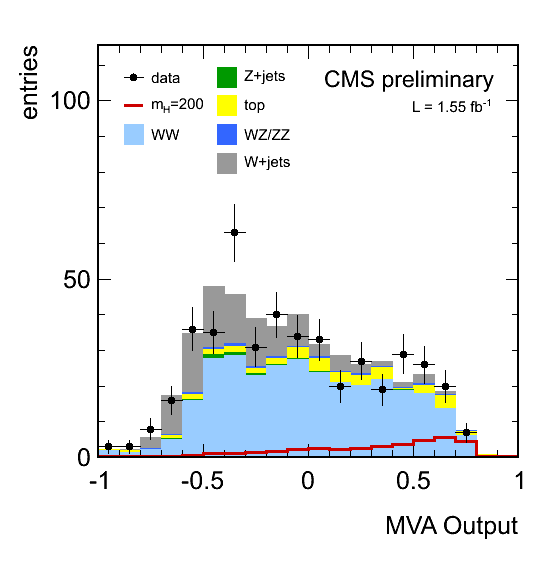
\includegraphics[width=.40\textwidth]{lp_figures/histo_mva_200_0j_of.png}}
\subfigure[]{
\centering
\label{subfig:lp_mva_200_0j_sf}
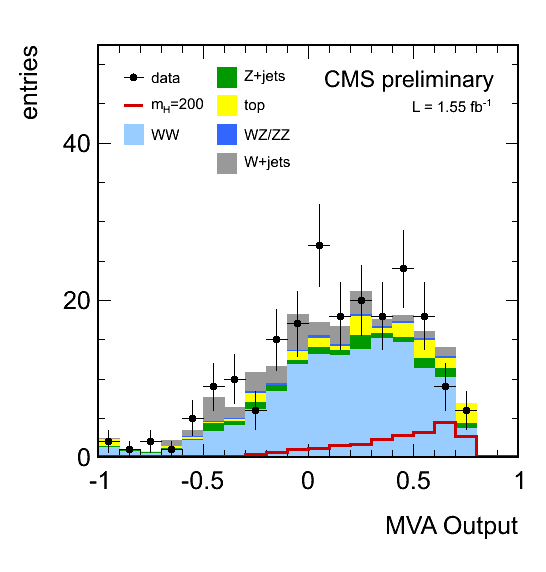
\includegraphics[width=.40\textwidth]{lp_figures/histo_mva_200_0j_sf.png}}\\
\subfigure[]{
\centering
\label{subfig:lp_mva_200_1j_of}
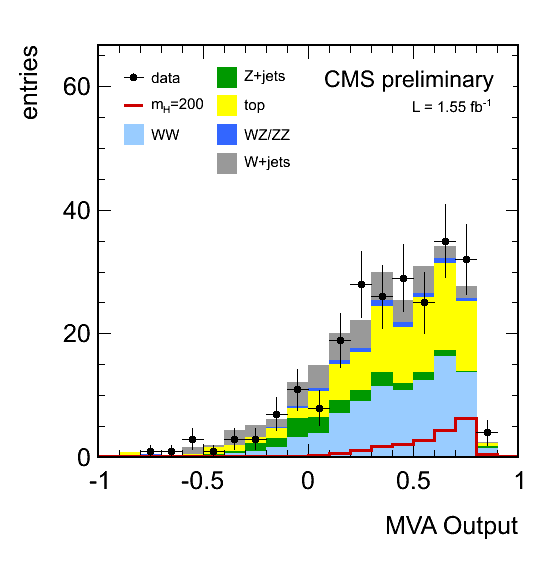
\includegraphics[width=.40\textwidth]{lp_figures/histo_mva_200_1j_of.png}}
\subfigure[]{
\centering
\label{subfig:lp_mva_200_1j_sf}
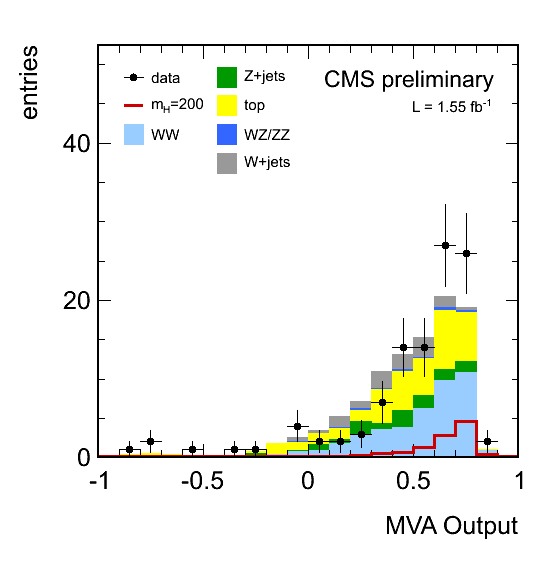
\includegraphics[width=.40\textwidth]{lp_figures/histo_mva_200_1j_sf.png}}
\caption{
MVA output for $m_H$=200 GeV LP analysis: 
0-jet OF \subref{subfig:lp_mva_200_0j_of},
0-jet SF \subref{subfig:lp_mva_200_0j_sf},
1-jet OF \subref{subfig:lp_mva_200_1j_of},
1-jet SF \subref{subfig:lp_mva_200_1j_sf}
.}
\label{fig:lp_mva_200}
\end{figure}

\clearpage
